\chapter{Anatomizing Smartphone Application Performance}
\label{chap:app}

Unlike traditional Internet-based applications, whose performance is mostly constrained by the wired network, network application performance on smartphones with limited physical resources also heavily depends on factors including hardware and software on the phone as well as the quality and load of wireless link. Understanding the application performance on smartphones is important for the purpose of assisting consumers in choosing carriers and phones and guiding application developers in designing intelligent software. Moreover, cellular network operators and smartphone hardware and software vendors can use this knowledge to optimize networks and phones for better end-user experiences. Similarly, content providers can leverage this knowledge to better customize content for mobile users. However, this task is quite challenging since the performance of network applications on smartphones is poorly understood before our study, due to a lack of a systematic approach for controlled experiments and comparative analysis. We believe this work fills this gap.

We focus on developing systematic methodology for measuring and analyzing 3G network performance as well as smartphone application performance. We make it relevant to end users by studying real applications directly on the phone platforms. Our approach differs inherently from most previous work of using laptops equipped with 3G data cards in three ways: (1) We measure the performance of applications rather than that of the low-level protocols. Prior work has shown that application performance often significantly deviates from protocol performance~\cite{Zhuang:A3:Mobicom2006}. We target the pervasive web browsing, streaming video, and VoIP applications that most end-users care about; (2) We measure application performance on several common mobile devices. Application performance varies widely across devices due to differences in hardware and software, necessitating direct experimentation on smartphones instead of on laptops with wireless cards; (3) We study the application performance under real-world scenarios and quantify the performance of web browsing by evaluating commercial websites in addition to locally-constructed ones with replicated, real web content under our control. The latter setup helps dissect and analyze the individual factors that contribute to the overall web browsing performance.

In addition to shedding light on the overall application performance, we perform detailed analysis to identify and isolate
factors that impact user-perceived performance to help carriers,
phone vendors, content providers, and application developers gain 
insight. For example, for carriers, we infer various network-level 
problems, \eg high latency or high loss rate, which they can directly 
take action on. For phone vendors, we identify performance bottlenecks 
on the devices or issues associated with the content. These issues can
be resolved either independently or by cooperating with content 
providers. And for application developers, we evaluate factors such 
as the overhead of HTML rendering and JavaScript execution given a 
particular software configuration.

We comprehensively study the 3G network and application performance
for all four major U.S. wireless carriers including AT\&T, Sprint,
Verizon, and T-Mobile. We choose popular devices including iPhone,
Android G2 from HTC, and Windows Mobile phones from Palm, HTC, and 
Samsung for carrying out experiments. Our results show that their
performance varies significantly across network applications. In 
fact, even for the same network application such as web browsing, 
certain types of phones consistently outperform others due to the 
differences in factors such as downloading behavior, customized 
contents, and page rendering. The application performance also 
heavily depends on properties of carriers including DNS lookup, 
RTT, and loss rate.

We summarize our main observations from extensive experimentation:

\begin{enumerate}

\item The four carriers we studied demonstrate distinct 
characteristics in network performance in terms of throughput, RTT, 
retransmission rate, and time-of-day effect. For example, compared 
with T-Mobile and AT\&T's median of TCP retransmission rate of 
0\%, Sprint and Verizon have a higher median value of 0.7\%. 

\item TCP throughput, RTT, and retransmission rate vary widely even
for a single carrier in measurement taken at different times and 
locations, \eg downlink throughput ranges from 50 kbps to 4 Mbps for 
AT\&T, with the median value of about 1 Mbps.

\item The wireless delay in the 3G network dominates the whole
network path delay, \eg latency to the first pingable hop is around 
200 ms, which is close to the end-to-end Ping latency to landmark
servers distributed across the U.S.

\item Besides networks, devices heavily influence application 
performance. Given the same content and network condition, different 
devices exhibit vastly different webpage loading time, \eg the
page loading time of Samsung SCHi760 is consistently twice that of 
iPhone. 

\item Mobile devices can benefit from new content optimization
techniques like the data URL scheme, \eg~page loading time for 
GPhone can improve by 20\% in our experiments, despite 
its already good performance compared to other devices.
\end{enumerate}

\nsection{Methodology and Setup for Measuring Web Browsing Performance}
\label{sec:app.method}

In this section, we present our methodology and setup for measuring web browsing application performance over 3G networks. By analyzing the performance of web applications, we examine the effects of various factors on the overall application performance.

Unlike most previous works, we directly measure application 
performance on devices that consumers really use with 3G service 
provided by four major cellular carriers in the U.S., this helps us 
understand the client side factors and their impact on application 
performance. The novelty of our measurement methodology stems from 
our approach of approximately replicating the 3G network condition 
for controlled experiments using WiFi to enable reproducibility, 
and isolating the impact of each factor. These techniques are 
non-trivial given the complexity of mobile devices and network 
environment, and essential for eliminating interaction across factors. 

Web browsing is one of the most popular smartphone applications. The 
process of visiting a webpage can be quite complex given the dynamic 
nature of the content, often generated from JavaScript, resulting in 
multiple concurrent TCP connections. Content can also be customized 
based on mobile device and carrier network.

Web browsing performance depends on various factors, \eg~DNS lookup 
time, TCP handshake time, TCP transfer time, JavaScript execution 
time, and content size. To study the effect of these factors, we 
carefully design controlled experiments to modify a single factor 
at a time while keeping others the same. We first describe the metrics 
used to evaluate web browsing performance, followed by the controlled 
experiments to measure these metrics.

\nsubsection{Web Browsing Performance Metrics}
\label{sec:app.web_metrics}

\paragraph{Application loading time:} 
%It is the time between the first DNS packet and the last data packet containing payload from the server during a page loading. It reflects the overall performance perceived by a user. Note that a browser needs to further parse and render a webpage after it is loaded. This additional processing cannot be fully included in page loading time due to a lack of visibility of the browser internals. Nonetheless, this is still a key indicator of user-perceived performance when loading a webpage. 

\begin{figure}[t]
\centering
\IG{figures/mobisys12/net_cpu.eps}\\
\ncaption{Network and CPU trace for \WY in LTE}
\label{fig:cpu}
\end{figure}


To measure application loading time, we use CPU usage as an indicator. Figure~\ref{fig:cpu} shows co-located network and CPU trace of an Android device visiting popular website in its default browser in the LTE network. At time 0, when ${\sf GO}$ button is clicked, loading starts. Before $t_a$, CPU usage stays low most of the time given that UE has not finished downloading the HTML or JavaScript objects. Starting from $t_a$, CPU usage jumps to 100\% and remains a high average usage until $t_c$. We notice that network activity nearly stops after $t_b$, with only a few TCP {\sf FIN} packets for closing TCP connections afterwards, some even come seconds later, \eg at time 10.5 seconds. During the time between $t_a$ and $t_c$, UE is rendering HTML pages or executing JavaScript, and during the time between $t_a$ and $t_b$, UE is also downloading web objects in parallel.
% Compared with simple mobile version websites, this content-rich website is selected to show network and CPU activity more clearly.

We define $t_c$ to be the {\em application loading time} instead of $t_b$, since at $t_b$, UE has not fully rendered the contents for the user, though the download process is complete. We validate this by collecting video traces with a camcorder facing the screen of the phone. We replay the video at normal speed and manually mark the start time and the end time, when the website gets fully loaded and all UI activity indicators stop. We verify that $t_c$ is an accurate estimate for application loading time. We also define the average CPU usage between time 0 and $t_c$ to be the {\em CPU usage} for this application.

Compared with a previous approach for measuring web browsing performance by modifying and instrumenting WebKit~\cite{hotmobile.web}, our approach is more lightweight and easily extensible to other applications other then web browsers, with reasonable accuracy. One limitation of our approach is that it is not applicable for applications, \eg streaming video/audio and some game applications, whose CPU usage remains high after initial loading.

\paragraph{JavaScript execution speed:} Many webpages contain 
JavaScript, and hence JavaScript execution speed has significant
impact on page rendering time. 

%Page rendering time depends on the client execution speed.
%We use JavaScript execution time as a measure of client execution speed since a large portion 
%of webpage content consists of JavaScripts.


\paragraph{Page size:} The total number of unique bytes downloaded. 
It can be used to compute {\it average throughput} and to detect 
content variation and customization. 
%Page size is important to understand content customization
%for each platform. 
We found that in typical web browsing, even the same URL can have different 
page sizes when accessed from different platforms. We cope with this 
effect by taking snapshots of URLs and replicate their content on our 
local web server.

%\paragraph{Connection completion ratio} denotes the percentage of complete TCP
%connections. A TCP connection starts with a SYN packet and ends with a
%FIN packet, a RST packet, or 
%a timeout. We consider a connection to be complete if it ends with a FIN. 
%We discard a page download sample if its complete connection ratio is low 
%(\eg $<95\%$). 

%\paragraph{Loss rate \& RTT} are extracted from the trace for each TCP 
%connection. We aggregate the loss rate (denoted as $p$) and the 
%RTT of individual connections to produce an overall measure of network 
%performance of a page download. Given that TCP throughput can be modeled as 
%$\frac{MSS}{RTT\times\sqrt{p}}$ where $MSS$ is the maximum segment 
%size~\cite{Padhye:TCPModel:sigcomm2008}, 
%the download time of a connection of size $S$ can be estimated as 
%$\frac{S\times RTT\times \sqrt{p}}{MSS}$. Since the download time of a connection 
%is proportional to $S$, $RTT$, and $\sqrt{p}$, we use 
%$\frac{\sum(S_i \times RTT_i)}{\sum S_i}$ and 
%$(\frac{\sum{(S_i \times \sqrt{p_i})}}{\sum S_i})^2$ as the average RTT and loss 
%rate of a page download.
%\paragraph{Packet inter-arrival time}

\paragraph{Browser concurrency:} Most modern browsers support concurrent 
TCP connections to a single web domain. The maximum number of concurrent 
TCP connections to a domain varies across different browsers. Usually, 
higher concurrency enables better bandwidth utilization which in turn 
leads to shorter page loading time.


\paragraph{DNS lookup time:} A browser sometimes needs to look up the IP
address of a domain name before establishing a TCP connection with the
web server. Since the content of a webpage can be hosted in multiple 
domains, a browser may have to perform a DNS lookup for each domain. 

%DNS lookup time is important because DNS lookups can increase page loading time.
%Since DNS lookup requests are handled by local DNS (LDNS)
%servers, we also compute the average DNS lookup time as a measure of LDNS server 
%performance.

\paragraph{TCP handshake time:} Each TCP connection starts with a
three-way handshake during which no data is transferred. More TCP 
handshakes for a single page loading often lead to longer page loading 
time.

\paragraph{TCP idle time \& transfer time:} Given a TCP connection, 
an {\it idle period} is defined to be a period of at least $T$ second 
with no network activity. The remaining time periods within the 
connection are {\it transfer periods}. An idle period usually 
corresponds to the local processing delay or server processing 
delay. Given the limited CPU power and memory on smartphones, the 
TCP idle time is likely to be dominated by local processing delay, 
\eg between the receipt of a response and transmission of the next 
request, often caused by HTML rendering and JavaScript execution.

\nsubsection{Web Browsing Controlled Experiment Setup}
\label{sec:app.setup}

We select a list of 20 popular and representative URLs (based on Alexa Top 500 Global Sites~\cite{alexa}) including search engines, emails, online maps, social networking websites, \etc
For most of the URLs, we use their mobile versions, specially optimized for smartphone users, as opposed to desktop versions. To facilitate repeated experiments, we write a program to invoke browser to visit each URL in turn with an interval of 120 seconds. Such interval is expected to be large enough to complete the page download. We used \emph{Apache} 2.0 HTTP server for hosting the replicated websites. We collect packet traces on iOS and Android using {\em tcpdump} and on Windows Mobile phones using {\em netlog}. We verify that the CPU utilization caused by trace collection is under 5\%. All the experiments are repeated at least 10 times.

These websites are visited using smartphones via 3G networks. From the collected 
packet trace, we infer various metrics such as page loading time.
To study the effect of each factor influencing the web browsing
performance, we host static copies of these popular URLs on our 
local web server. The content is replicated to ensure that all the 
phones download the same content and all HTTP requests are sent to 
the local server. To control the network conditions, we uniformly 
use WiFi across all phones while varying one factor at a time. 
The WiFi link is lightly loaded and has stable throughput and RTT. 
To produce network conditions comparable to 3G, we artificially 
introduce delay and packet loss at our server. We study the impact 
of the following factors on web browsing performance:

\paragraph{Impact of network:} To study the effect of network
conditions on page loading time, we vary the RTT and loss rate 
on our server. To introduce artificial delay and loss, we ran a user-level program 
on the server. This program intercepts all packets destined to a 
particular IP address and injects delay and random packet loss. We 
controlled loss rate values from 0\% to 10\% and RTT values from 0~ms 
to 800~ms. These values cover the major range of loss rate and RTT 
values observed in 3G networks from our previous analysis. 

\paragraph{Impact of concurrency:} To study the effect of 
concurrency, we control the maximum number of concurrent TCP 
connections to a web domain on the server side by configuring the 
\emph{Apache} server with the help of the {\em mpm\_prefork\_module}.

Because a phone also limits the maximum number of concurrent connections per domain, we create a special webpage with 30 embedded objects in which each web object is hosted in a unique domain (a DNS alias) on the same web server. This effectively allows us to bypass the per-domain concurrency limit imposed by the phones. Note that this is necessary as we do not have the permission to directly modify the concurrency limit on the phone. For concurrency experiments, we use the RTT of 400 ms and the loss rate of 0\%. 

\paragraph{Impact of compression:} To study the tradeoff between 
network overhead and computation overhead, we configure our web
server into two modes, one uses compression, while the other does 
not. We compare the page loading time under these two modes.
Specifically, we use {\em SetOutputFilter}and {\em BrowserMatch} directives to specify whether compression is enabled for a specific type of browser, \ie compression is bypassed  by adding the following lines to the Apache config file:

\begin{lstlisting}
<Location />
	SetOutputFilter DEFLATE
	BrowserMatch Mozilla no-gzip
</Location>
\end{lstlisting}


We fix the loss rate at 0\% and vary the RTT from 0 ms to 800 ms. Our goal is to understand whether compression is beneficial under different network conditions.

\paragraph{Impact of JavaScript execution speed:} To evaluate 
JavaScript execution speed on different phones, we use a 
benchmark~\cite{sunspider} consisting of 26 different JavaScripts. 
The benchmark is hosted on our web server and accessed by phones 
via WiFi so that the downloading time is negligibly small. We 
measure the total execution time of these JavaScripts. 

\paragraph{Impact of the data URL scheme:} We also study the effect 
of the data URL scheme~\cite{rfc2397}, a recently-proposed mobile 
webpage design technique. We compare the time to load a webpage 
constructed using and without using the data URL scheme. 
Specifically, we construct a webpage with 20 images; 10 of them are of size 18KB and the remaining 10 are of size 0.241KB. We create two versions of this webpage, one with links to download the images and the other with the images embedded in the webpage itself. We could not carry out this experiment for Windows Mobile phones since IE does not support the data URL scheme in 2009.


\nsubsection{Analysis Methodology}

We next describe how to analyze the traces collected from controlled
experiments to compute the desired metrics. We calculate the page 
loading time of each URL as defined in Section~\ref{sec:app.web_metrics} 
and the average page loading time of all the selected URLs. To measure 
JavaScript execution time, we modify the JavaScripts to display their 
execution time when their execution finishes. We use the
{\em average concurrency} as a measure of browser concurrency. The
average concurrency of a page loading is calculated by dividing the 
total duration of all the TCP connections by the page loading time. 

For each TCP connection, TCP handshake time is calculated as the time
between the first \emph{SYN} and \emph{SYN-ACK} packets. TCP idle time 
is measured by scanning the connection for durations of more than 
\emph{T} seconds of no network activity. \emph{T} should be larger 
than the maximum RTT values. In our analysis, we choose \emph{T = 1} second, as we have seen that in cellular networks, even for 3G networks, RTT is smaller than 1 second in 99\% of the cases. Thus, if there
are no network activities for 1 second or more, the phone should 
be busy with some local processing, \eg rendering HTML pages or executing JavaScripts.
TCP transfer time is what remains for the connection excluding handshake and idle time. 
We also calculate the response time of all the DNS lookups $T_{dns}$. 

%given the difficulty of
%estimating the total time for the three-way handshake. 

Since each web browsing session often consists of multiple concurrent
TCP connections, to estimate the contribution of each factor to the 
overall performance, we logically serialize all DNS lookups and TCP 
connections. This is possible for mobile web browsing since no HTTP 
pipelining is observed on any phones. After serialization, we get a 
total time $T_{total}$ which is the sum of each connection's duration. 
Assuming the actual page loading time is $T^{*}_{total}$, the
normalized DNS lookup time $T^{*}_{dns}$ is calculated as
$T^{*}_{total} * T_{dns} / T_{total}$. This metric shows the 
overall weight of DNS lookup in the actual page loading time. The
normalized TCP handshake time, TCP idle time and TCP transfer time 
are calculated in a similar way. 
%We also get a temporary total time for
%DNS lookup ($T_{dns}$) by adding up the response time of each DNS
%lookup.
%For concurrent DNS lookups with the same request, only the response time of the first DNS
%request is counted because subsequent DNS lookups will not affect performance.	



\nsection{Web Browsing Performance Study}
\label{sec:web}

%%Motivation of the work
Given the previous discussions on the performance of 3G networks, we 
now examine one of the most popular applications on smartphone, 
namely web browsing, in addition to two other popular mobile 
applications, streaming video and VoIP in \S\ref{sec:other}. Note 
that many factors jointly determine user perceived performance, as 
an application may not fully utilize available network bandwidth due 
to limited processing power or memory on the 
phone~\cite{Zhuang:A3:Mobicom2006}.

%%highlights of our findings
Our study shows that the available 3G bandwidth is often not fully
utilized for web browsing, and several modifications can be applied 
to current web browsers on smartphones to make better use of
available network resources, \eg increasing the limit on concurrent
TCP connections per domain, optimizing JavaScript engines \etc We 
also evaluate the effectiveness of a few content optimization 
techniques, including compression and the recently-proposed data 
URL scheme~\cite{rfc2397}.

In the following, we study the impact of network condition, browser
concurrency, compression, and JavaScript execution speed on web 
performance. We then break down the page loading time into several 
major components and identify the performance bottleneck for some 
mobile devices (\S\ref{sec:web_real}).

%network
\nsubsection{Network Effects on Web Browsing}
\label{sec:web_net}

\begin{figure*}[t]
\centering
\begin{tabular}{cc}
\IGM{figures/mobisys10/web_rtt.eps} &
\IGM{figures/mobisys10/web_loss.eps}\\
\small{(a) Effect of round trip time on web browsing} &
\small{(b) Effect of downlink packet loss rate on web browsing} \\
\IGM{figures/mobisys10/web_para.eps} &
\IGM{figures/mobisys10/web_compress.eps}\\
\small{(c) Effect of parallelism on web browsing} & 
\small{(d) Effect of compression on web browsing} \\
\end{tabular}
\ncaption{Factors impacting web browsing performance}
\label{fig:web_factor}
\end{figure*}

To understand how network condition affects web browsing, we fix the 
web content, server configurations, browser concurrency and only vary 
the network condition. We emulate the 3G network condition by 
injecting packet delay and loss on the WiFi network path as described 
in \S\ref{sec:method}.

Figure~\ref{fig:web_factor}(a) shows that page downloading time increases
linearly with the RTT between smartphone and our local web server. 
The downloading time is computed by averaging across 20 replicated 
URLs, with each URL visited 3 times. This is expected as throughput 
is inversely proportional to RTT. No additional packet loss is 
introduced since packet loss is observed to be rare in 3G 
networks, as shown in the previous section. The base RTT in our WiFi network is between 30 ms and 50 ms. 
The x-axis in Figure~\ref{fig:web_factor}(a) shows the actual RTT 
after injecting extra delay. We can observe that under the same 
network condition, downloading time varies across phones though the 
relative ranking remains consistent. Note that web browsing cannot 
fully utilize the available network bandwidth, due to the overhead
imposed by page execution 
and rendering on the phone.

Figure~\ref{fig:web_factor}(b) shows the effect of varying downlink
packet loss rate for a fixed RTT value of 400 ms. Again the ranking 
in downloading time across phones is consistent. For small packet 
loss rate, \eg~2\%, there is little performance degradation. However, 
with 10\% loss rate, the page downloading time increases up to 35 
seconds. In summary, smartphone web browsing performance heavily 
depends on network delay and loss conditions.


%parallel
\nsubsection{Concurrent TCP Connections}
\label{sec:web_parallel}

3G network's downlink throughput as measured normally ranges from 500 
kbps to 1 Mbps for the carriers we studied (Figure~\ref{fig:net.general}(a)). 
We used the phones to visit the chosen URLs and found that the average 
throughput is only between 20 kbps and 50 kbps, indicating that 
more concurrent TCP connections can potentially improve web browsing 
performance.

Current web browsers on smartphones already allow concurrent 
connections. In browser's settings, there is a parameter specifying 
the maximum number of concurrent TCP connections per domain. On 
Windows Mobile phones, it is a registry value named 
{\em MaxConnectionsPerServer} with a default value of 4. When we 
set the value to be smaller than 4, we observe decreased 
concurrency. However, when we increase the value to be larger than 
4, the concurrency does not increase accordingly. This implies there 
exists another setting on maximum allowed concurrency per domain, 
which we cannot configure. For iPhone and GPhone, we are unable to 
set this parameter either. We design controlled experiments to measure 
the default concurrency setting on different platforms and found it 
to be 4 for all the phones studied. 

We also found that no HTTP 
pipelining support is present on these platforms.
%Analyzing the packet traces we collected, we found that TCP connection reuse is common,however, 
Web objects are fetched sequentially within a persistent connection,
and browser will not send a new HTTP request before data transfer
of the previous request completes. %Studying the impacts of
%adding HTTP pipelining support to smartphone browsers is one of
%our future directions.
We analyzed the 20 popular URLs and found that there are 10.8 images 
embedded in each page on average, along with several other types of 
embedded objects, such as JavaScript, CSS files, \etc Those websites 
which do not have a mobile version, tend to have even more objects. 

%Parallelizing the download of objects hosted 
%on different servers will allow the browser to make
%better use of the link capacity since the TCP establishment
%time of each TCP flow can be in parallel with 
%the downloading of other objects and multiple concurrent TCP flows
%would have a better chance to saturate the link.
%However, if too many connections are opened concurrently, given
%the limited resources on smartphones, such as CPU and memory, and
%the limited bandwidth for 3G networks, the overall performance of 
%Web browsing could be degraded by the context switching overhead
%and the extra workload to manage and maintain those parallel connections.
%When two objects are hosted on the same server, the browser also has
%a decision to make: to download them one after another by reusing the same
%TCP connection, or to download them concurrently by having two concurrent
%TCP connections to the server. From the server's perspective, the approach
%of reusing connection is preferred, since the server's workload is smaller. 
%However, determining which approach of the two can achieve better performance on
%smartphones is not trivial, and the answer is dependent on the CPU and bandwidth
%utilization, as well as the object size \etc 
%If simply downloading two large objects, 
%concurrent connection approach would have better performance;
%while reusing connection approach could be better if the CPU and bandwidth utilization
%on smartphones is already very high, or if the objects are relatively small in size,
%because in this case, the overhead of an extra TCP connection establishment will
%be less negligible.

%To understand whether the concurrency setting is appropriately 
%configured to optimize web browsing performance, 
%This suggests the 
%benefit of higher parallelism than the default setting.

%The study on the default settings of today's mobile browsers
%and the characteristics of today's mobile websites shows some
%possibility of improving mobile Web browsing performance by
%tuning related parameters. We argue that, even though
%the CPU, memory and bandwidth resources are limited on 
%smartphones, properly increasing the parallelism in
%today's mobile browsers' default settings may still improve
%the Web browsing performance.

To understand how concurrency affects web browsing performance, we
devised a set of experiments, with results shown in 
Figure~\ref{fig:web_factor}(c). %Since the default setting for max
%parallel connections per server on all browsers studied is 4, 
We first vary the maximum concurrent connections allowed at the server 
side from 1 to 4. We observe a significant performance degradation 
across all platforms with more restricted concurrency. Under the 
restriction of a single connection per domain, web browsing is 3.5 
to 4.5 times slower compared to that under the default setting. This 
indicates that today's mobile browsers already benefit much from 
concurrency.

To understand whether further increasing concurrency will improve 
performance, we make use of DNS aliasing 
(Section~\ref{sec:app.setup}) to bypass the concurrency limit on 
the phone since we are unable to change this setting directly.
%With the help of this technique, the client side
%parallelism limit is removed and the maximum parallelism
%is only restricted by the content, which
%corresponds to the \emph{OPT} results in
%\comment{In Figure~\ref{fig:web_factor}(c), OPT stands for the cases 
%that we do not limit the maxmium allowed concurrent connections at the 
%server side.}
Figure~\ref{fig:web_factor}(c) shows that the phones can indeed
attain a higher level of concurrency. For example, iPhone and G2 
can establish up to 9 concurrent connections for some content-rich 
URLs. The concurrency for other phones are slightly lower (6 to 7), 
likely due to their slower rendering and execution speed.
%We can also observe that without
%the client side parallelism limitation, the Web browsing
%performance can be further improved by 30\%. 
Generally, an improvement of 30\% is observed when concurrency limit
on the phone is removed.
%\comment{compare against the page downloading 
%time when the maximum observed concurrency is 4}. %While the optimal concurrency setting
%is dependent on factors such as content, execution speed, and network
%conditions, 
This means that given the selected popular URLs, and given 
current network condition (with RTT of 400 ms), the default
concurrency setting on mobile browsers appears to be too
conservative. Allowing higher concurrency can help phones
make better use of available bandwidth and decrease page downloading time.



%%%%%%%%%%%%%%%%%%%%%%%%%%%%%%%%%%%%%%%%%%%%%%%%%%
%%% URL analysis table
\begin{table*} [t!]
\begin{center}
\scriptsize
\begin{tabular}{|c|c|c|c|c|c|c|c|c|c|}\hline
URL & Text\footnotemark[1] & Image & Size(KB) & Original(KB)\footnotemark[2] & Compress\footnotemark[3] & GZIP & Lines\footnotemark[4] & Redirect & Sever IPs\\
\hline
\hline
www.google.com & 4 & 1 & 79.2 & 77.6 & 2.56 & \checkmark & 14 & - & 2\\\hline
m.bing.com & 4 & 3 & 42.9 & 218.1 & 1.46 & - & 2 & - & 1\\\hline
maps.google.com & 6 & 10 & 479.8 & 656.0 & 2.78 & \checkmark & 8 & - & 4\\\hline
mapquest.com & 6 & 13 & 135.1 & 1326.35 & 1.96 & \checkmark & 752 & 2 & 6\\\hline
xhtml.weather.com & 22 & 9 & 41.4 & 977.3 & 2.53 & - & 70 & 4 & 2\\\hline
%www.wikipedia.org & 2 & 14 & 125.8 & 1.92 & \checkmark & 522 & - & 2\\\hline
m.youtube.com & 5 & 3 & 77.6 & 490.1 & 2.34 & \checkmark & 231 & - & 3\\\hline
m.ebay.com & 4 & 3 & 58.6 & 484.0 & 2.17 & - & 1 & - & 1\\\hline
m.facebook.com & 4 & 1 & 19.7 & 399.1 & 2.81 & \checkmark & 7 & 2 & 2\\\hline
m.myspace.com & 3 & 2 & 14.6 & 600.2 & 2.6 & \checkmark & 98 & 1 & 2\\\hline
m.fox.com & 4 & 26 & 306.6 & 2083.0 & 1.16 & \checkmark & 297 & - & 4\\\hline
mobile.craigslist.org & 3 & 0 & 113.8 & 113.8 & 3.58 & \checkmark & 652 & - & 1\\\hline
\end{tabular}
\\
\begin{tabular}{l}
{\scriptsize $^1$This column shows the number of text objects including HTML, JavaScript and CSS files}\\
{\scriptsize $^2$This column shows the total size of the original website for each mobile URL, for example, www.bing.com for the row of m.bing.com}\\
{\scriptsize $^3$This column shows the compression ratio for mobile URLs, total size in no compression mode / total size in compression mode}\\
{\scriptsize $^4$This column shows the total number of lines in the index page indicating whether minification is used}\\
\end{tabular}
\ncaption{Characteristics of today's popular mobile websites}
\label{tab:url}
%\end{footnotesize}
\end{center}
\end{table*}


%compression
\nsubsection{Content Compression}
\label{sec:web_compress}
%By add two header fields \texttt{Content-Encoding} and \texttt{Accept-Encoding}, HTTP/1.1 supports content compression. To deploy the compression, HTTP interactivity between the request and response is introduced. In the interactivity, The browser declares the acceptable compression algorithms in \texttt{Accept-Encoding} field in the HTTP \texttt{GET} request like:
%\newline \noindent
%\texttt{
%GET / HTTP/1.1\\
%Accept: */*\\
%Accept-Language: en-us\\
%Accept-Encoding: gzip,deflate\\
%User-Agent: Mozilla/4.0 (compatible; MSIE 6.0; Windows CE; IEMobile 7.11) VZW:SCH-i760 PPC 240x320\\
%Connection: Keep-Alive\\
%}
%When the server replies, the HTTP header looks like:\\
%\noindent
%\texttt{
%HTTP/1.1 200 OK\\
%Content-Type: text/html; charset=UTF-8\\
%Content-Encoding: gzip\\
%Content-Length: 3228\\
%}
%In the above example, the browser tells the server that it supports content encoding in gzip, or deflate. 
%For each HTTP request, the client informs the Web server whether
%compression is supported and the server then decides whether and how
%to compress various Web objects. 

Compression can dramatically reduce web content size. For text objects, 
such as HTML, CSS, JavaScript, PHP, \etc, the object size can be reduced 
by around 70\%. Usually, a web server does not compress image objects.
We calculate the compression ratio for the popular URLs in column 
{\em Compress} of Table~\ref{tab:url}, showing that the content size 
can be reduced by more than 50\% for most of the URLs we studied.

While compression reduces the bytes transferred over the network, 
decomression will increase computation overhead on the phone. To
understand this tradeoff, we vary RTT covering the measured range
and compare the web browsing performance in compressed and 
uncompressed modes. In Figure~\ref{fig:web_factor}(d), we exclude the 
results for HTC and Palm phones as they show similar trends. We 
observe that compression consistently helps to improve web performance,
irrespective of the RTT values. It is especially helpful under 
poor network condition.
%\comment{because the network more likely becomes 
%the bottleneck than compresssion computation at that time}.
For example, it reduces iPhone's page 
downloading time by 30\% when RTT is 800ms. 

%In Table~\ref{tab:url}, we listed the webpage size and the compression ratio for some popular mobile websites. Take {\em m.facebook.com} as an example of the smaller webpage, its compression ratio is as high as 2.81, but its total page size is only 19.7 KB, while {\em m.fox.com} has a small compression ratio 1.16, but a higher compression space due due to the larger content size 306.6 KB.
%
%In order to understand the impact of compression on mobile platforms, we controlled the compression mode of {\em Apache} on our server, and compared the page downloading time under two cases when we enable or disable the compression. In the comparison, we also artificially controlled the RTT changing from 0ms to 900ms so that it covered the 3G throughput range. 
%In summary, we verify that compression helps improve Web browsing
%performance by up to 30\%. There is still such opportunity remaining
%as we observe in the actual 3G Web browsing experiments, some text
%content from some servers are sent as uncompressed, as discussed later
%in \S\ref{sec:web_server}.

%We think enabling compression for transferring textual files is a
%good practice for mobile Web servers.



%js
\nsubsection{JavaScript Execution}
\label{sec:web_js}

\begin{figure}[t]
\centering
\IG{figures/mobisys10/web_js.eps}\\
\ncaption{Script execution speed for different platforms in 2009}
\label{fig:web_js}
\end{figure}


%Webpage consists of HTML tags which describe how the text should be formatted when a browser displays it on the screen. 
%These tags act as instructions which are interpreted by browser and merged with the text to produce a formatted display.
%This process is called HTML rendering. A significant number of HTML tags are JavaScript tags.
Given the limited processing power on smartphones, HTML rendering 
and JavaScript execution may become the bottleneck for web browsing. 
Several factors jointly determine the page processing speed, 
including CPU frequency, memory, OS, and browser.
%(the actual CPU frequency is also
%related with the specific dynamic frequency scaling policies
%of the device), 
Even for the same OS, such as Windows Mobile 6.1, phone vendors 
can have different builds for different models of phones.

We measure JavaScript execution time on different phones using a
benchmark consisting of 26 different JavaScripts~\cite{sunspider}.
Figure~\ref{fig:web_js} shows the total time taken to execute 
the benchmark on different phones measured in 2009. The results demonstrate that
execution time is 20$\sim$80 times longer on smartphones than on desktop
computers. Among the smartphones, G2 has the best performance 
followed by iPhone. For example, G2 is 3 times faster than the HTC
phone. Such performance gap helps explain the differences in the
page loading time of G2 and iPhone compared to that of the Samsung 
and Palm phones under the same network conditions in 
Figure~\ref{fig:web_factor}. Large JavaScript execution time leads 
to more TCP idle time and under-utilization of network bandwidth.

This experiment shows that network is not the only bottleneck for 
web browsing performance. Phone itself also plays a major role, 
underscoring the necessity of measuring application performance
on real smartphones. Web designers should avoid using complex
JavaScripts when building mobile versions of their websites. 

\begin{figure}[t]
\centering
\IG{figures/mobisys12/js.eps} \\
\ncaption{JavaScript execution speed comparison}
\label{fig:js}
\end{figure}

We revisited the JavaScript execution experiments in 2011, as shown in Figure~\ref{fig:js}. We consistently use the same benchmark~\cite{sunspider} (version 0.9) to quantify the JavaScript execution speed. In Figure~\ref{fig:js}, the test results on the same G1 phone in 2009 and in 2011 are very close, validating that the benchmark of that version has not changed since 2009.

From 2009 to 2011, iOS has a speedup of 29.88 for iPhone~4 and 51.95 for iPhone~4S, while 21.64 for Android and 22.30 for Windows Phone. And the gap between smartphone and computer has dropped to 5.5$\sim$23.1 times in JavaScript execution speed. Possible reasons for this improvement include fast CPU, larger memory, and better OS and application software for smartphones.


%Server configuration and content optimization
\nsubsection{Server Configuration and Content Optimization}
\label{sec:web_server}

Server configurations and content optimization are important factors 
for web browsing performance. One type of server configuration is 
the maximum concurrent connections with a client. In 
\S\ref{sec:web_parallel}, we found that mobile browsers set a
default concurrency limit of 4 per domain. However, we did not observe 
any web servers limit the concurrency per client to be smaller than 4, 
likely because servers have the incentives to attain good web browsing 
experience. The compression configuration is similarly important, with 
the identified setting of the URLs studied shown in the {\em GZIP} 
column in Table~\ref{tab:url}. Despite the fact that compression almost 
always improves web browsing performance (\S\ref{sec:web_compress}), 
we found some websites do not enable it by default.

Various content optimization techniques also help improve web 
browsing performance on smartphones. Most popular websites already 
customize their contents for mobile users, with more concise texts 
and fewer and smaller images, \eg via code 
minification~\cite{minification}, image scaling, \etc We study in 
particular code minification which refers to the elimination of 
redundant characters, such as spaces, tabs, line breaks, \etc The 
size reduction varies from 5\% to 25\% for the URLs studied. 
Column {\em Lines/index} in Table~\ref{tab:url} shows the number of 
lines in the index page of a website, providing a hint for whether 
minification is used. The number of lines will be small for index
pages treated with minification. It seems that half of the URLs use 
this technique to optimize their contents.


\begin{figure}[t]
\centering
\IG{figures/mobisys10/web_dataurl.eps}\\
\ncaption{Evaluation for data URL scheme}
\label{fig:web_dataurl}
\end{figure}

Another type of optimization helps reduce the number of HTTP 
requests used to fetch contents, including the data URL 
scheme~\cite{rfc2397}, CSS3, \etc The general idea is to eliminate 
TCP connections and HTTP requests for small objects, such as the 
corner image of a page. 
%comment{Since TCP has slow-start behavior, it is inefficient to download a small object using an extra TCP connection.}
We set up a controlled experiment to demonstrate the effectiveness of the data URL scheme, under which small images are integrated with the main HTML page rather than linked as separate objects (\S\ref{sec:app.setup}). 
%When a browser downloads the HTML page, the images 
%are downloaded together.
In our experiment, we found that the images are actually 1.3--1.5 
times of its original size under the data URL scheme. 
%comment{Nonetheless, due to the elimination of TCP connections and HTTP request overhead, data URL scheme still helps.}
Figure~\ref{fig:web_dataurl} shows that it cuts page loading
time by about 20\%.

The data URL scheme has not been ubiquitously supported. In fact, 
%comment{among the phones we studied},
only the browser of iPhone and G2 supports it. We also did not 
observe any URLs we studied adopt this technique, possibly due to the 
concern of a lack of browser support. Without browser support, the 
image represented by the data URL scheme will be displayed as a 
default error image.

Redirection (HTTP response code 301 and 302) is another issue which
may adversely impact web browsing performance. For mobile web browsing, 
this issue becomes more pronounced given the large RTTs in 3G networks. 
In column {\em Redirect} of Table~\ref{tab:url}, we found that some 
websites have multiple levels redirections. For example, 
\url{m.weather.com} will be redirected to \url{xhtml.weather.com} and 
then to \url{mw.weather.com}. In some cases, users are redirected to 
another URL which is quite similar to the original one. In other 
cases, web objects have been moved to a new location, and the original 
URL simply redirects the incoming requests to the new location. We 
think some of these redirections are unnecessary and can be eliminated 
with better webpage design.

%a.png actual 247 data 378  1.5
%b.png actual 18319 data 24460  1.3
%
%about 1.33 times page size
%original: 187K vs. 248K  (data url)
%but data url benifit from html compression, for original pages, images can't benifit from gzip
%
%loading time:
%Data url vs. Original
%iPhone: 2.98 vs. 3.87
%G2: 1.6 vs. 1.99
%Samsung / Palm: doesn't support
%


%\comment{2. write about redirection. 301 Moved Permanently; 302 Moved Temporarily(original describing phrase; 302 Found; (1 or multiple redirection, waste of bandwidth though small(many users), waiting time, several RTT}
%\comment{example for redirect: www.google.com no redirection but different content see table 3}




%breakdown
\nsubsection{Understanding Bottleneck Factors for Web Browsing}
\label{sec:web_real}

%Studying Web browsing on smartphones using 3G networks visiting
%real mobile websites, we can conclude that 3G network performance is not
%the only bottleneck. Content optimization for mobile
%users, server configurations, as well as client execution speed
%are also important factors.

\begin{figure*}[t]
\centering
\begin{tabular}{c}
\IG{figures/mobisys10/url10.eps} \\
\small{(a) Web browsing breakdown for \url{m.ebay.com} (\emph{URL a})} \\
\IG{figures/mobisys10/url19.eps}\\
\small{(b) Web browsing breakdown for \url{mapquest.com} (\emph{URL b})} \\ 
\end{tabular}
\ncaption{Web browsing anatomy for two popular mobile websites}
\label{fig:web_real}
\end{figure*}

Figure~\ref{fig:web_real} shows the case study for two groups of
URLs listed in Table~\ref{tab:url}. \emph{Group A} corresponds to 
the URLs that have concise and simple contents, \eg \url{m.ebay.com}
(\emph{URL a}) contains 7 objects with a total size of 58.6 KB.
Many of these websites are search engines or portals to social
networking sites, including \url{www.google.com}, \url{m.bing.com},
\url{m.myspace.com}, and \url{m.facebook.com}. \emph{Group B} 
consists of websites with rich contents, \eg \url{mapquest.com}
(\emph{URL b}) has 19 objects with a total size of 135.1 KB. Other
websites in the group include online map (\url{maps.google.com}), 
information exchange (\url{mobile.craigslist.org}), and news 
(\url{m.fox.com} and \url{m.cnn.com}).

There are two sets of data in Figure~\ref{fig:web_real}. One set is
collected when each smartphone visits the real URLs via 3G networks. 
To eliminate the differences in downloaded contents and network 
conditions, each phone also visits the replicated URLs via WiFi with
an RTT of 400 ms to emulate the typical 3G network conditions.

It is clear that all smartphones experience smaller page loading
time for the simple URL in Figure~\ref{fig:web_real}(a) compared with 
that for the content-rich URL in Figure~\ref{fig:web_real}(b). We 
break down the page loading time into four parts: TCP transfer, 
TCP idle, DNS lookup, and TCP handshake. The size of \url{mapquest.com} 
is larger than that of \url{m.ebay.com}, resulting in longer TCP 
transfer time. Moreover, \url{mapquest.com} contains more contents 
to render and more complex JavaScripts to execute, leading to longer 
TCP idle time. The DNS lookup time and TCP handshake time contribute
to less than 10\% of page loading time, which are negligible.

%so we can conclude that the
%bottleneck consists mostly of network performance and client
%processing speed.

%Even though URL b has more objects to download than URL a,
%if all objects are hosted on the same server, there will be
%no extra DNS lookup overhead. Also since TCP connection to the
%same server will be reused to download multiple objects,
%the TCP handshake overhead will be small.
%The reason for URL b's relatively high TCP handshake overhead
%and DNS lookup overhead is due to the fact that
%the objects in URL b is hosted on 6 different servers, while
%only 1 server host URL a. DNS lookup of browsing URL b includes
%www.mapquest.com, content.mqcdn.com, o.aolcdn.com, o.sa.aol.com.
%From the domain names, we can infer that URL b already benefit
%from the use of content delivery network (CDN), however,
%this benefit is reduced when multiple CDN servers are involved
%while causing DNS lookup overhead and TCP establishment overhead
%since TCP connection cannot be reused across multiple servers.
%There is a tradeoff between hosting contents on the same server
%and on different servers, since hosting contents on different
%servers will allow the client to benefit more from parallelism.
%Based on our observations, it depends on the actual contents.

We further observe that the Palm (Sprint), Samsung (Verizon), and 
HTC (AT\&T) phones experience much longer page loading time for
\url{mapquest.com} compare to iPhone (AT\&T) and G2 (T-Mobile). 
This is likely due to their slower JavaScript execution speed,
as shown in Figure~\ref{fig:web_js}. 
%larger slow down
%as a result of the differences caused by network and client factors
%for content-rich URLs compared with simple URLs.

%compared with in Figure~\ref{fig:web_real}(a). 
%Based on the results in Figure~\ref{fig:timeofday}(a),
%we already know that T-Mobile and AT\&T supply relatively 
%better 3G downlink capacity compared with Sprint and Verizon.
%Since URL b has more data to transfer, the impact of network
%performance difference becomes more obvious.
%Similarly, in Figure~\ref{fig:web_js}(a), we know that
%Samsung/IE and Palm/IE perform worse than iPhone/Safari and
%G2/Browser, the performance gap will be more obvious
%for URLs that have richer contents, such as URL b.

%The reason for comparing with WiFi experiments visiting hosted content
%on our local server as shown in Figure~\ref{fig:web_real} is to
%account for differences in content and network conditions. Content can
%differ even for the same URL due to server side content optimization
%based on user agent. WiFi also eliminates the difference in network
%condition across devices. 
In the WiFi experiments, all the phones download the same contents and 
experience the same network conditions. As a result, the TCP transfer
time differences among all phones are small. However, we can still 
observe significant page loading time differences, mostly due to the
gap in TCP idle times. We further note that their relative ranking is 
consistent with the ranking of JavaScript execution speed in 
Figure~\ref{fig:web_js}.


\begin{figure*}[t]
\centering
\IGL{figures/mobisys12/app_compare.eps}
\\
\small
\begin{tabular}{l}
$^\star$The loading time is normalized by the maximum loading time observed in this figure,\\
and similarly for total energy
\end{tabular}
\ncaption{Loading time, CPU usage and energy consumption analysis on mobile applications}
\label{fig:app.compare}
\end{figure*}

The previous part of the study was carried out in 2009. Along with improvements in mobile client processing power, LTE technology significantly increased network speed. So we perform another case study of a few popular applications to understand the impact of network speed and processing power enhancement on user-perceived performance in 2011.

With the measurement methodology discussed in Section~\ref{sec:app.web_metrics}, we compare loading time, CPU usage, and energy consumption for several popular applications in Figure~\ref{fig:app.compare}. We collect both network and CPU traces on an Android device with LTE data access. Specifically, we select the default browser, YouTube, NPR News and Android Market as our sampled applications given their popularity. For the default browser, we choose two different usage scenarios, \ie visiting mobile version of \url{google.com} representing a simple website and visiting non-mobile version of \url{yahoo.com} representing a content-rich website. We name the two browser usage scenarios as \WG and \WY, respectively. While for the other applications, we click the application icon until the initial page is fully presented to the user. We make sure the cache is cleared before each experiment. These usage scenarios are representative for web browsing and other similar web-based applications, different from audio and video streaming applications.

First, loading time comparison shows that LTE and WiFi have comparable user-perceived delay for the studied scenarios, and 3G lags behind with 50\%$\sim$200\% larger response time. The application loading time for LTE slightly lags behind WiFi. On one hand, given that promotion delay is counted into the loading time, LTE has larger $T_{pro}$. On the other hand, though LTE has faster throughput than WiFi with throughput tests, its RTT is slightly larger. To understand why RTT matters more than throughput for the usage scenarios in Figure~\ref{fig:app.compare}, we analyze the object size statistics for different applications in Table~\ref{tab:app.size}.

\begin{table}[t]
\begin{center}
\begin{tabular}{|c|c|c|c|c|}\hline
Application & Total payload & Maximum object size & \# objects & Average size \\\hline
Website G & 160.7KB & 87.6KB & 11 & 14.6KB\\\hline
Website Y & 509.9KB & 124.2KB & 59 & 8.6KB\\\hline
YouTube & 449.1KB & 109.4KB & 33 & 13.6KB\\\hline
NPR News & 306.2KB & 169.5KB & 9 & 34.0KB\\\hline
Market & 599.7KB & 145.4KB & 17 & 35.3KB\\\hline
\end{tabular}
\ncaption{HTTP object statistics}
\label{tab:app.size}
\end{center}
\end{table}

In Table~\ref{tab:app.size}, across all scenarios, the maximum object size is 169.5KB for NPR News and the average object size is at most 35.3KB for Android market. Especially for \WY, there are 59 HTTP objects with an average size of only 8.6KB. Due to TCP slow start, these objects are far from saturating the link capacity for either LTE or WiFi. Persistent TCP connections are observed to transfer multiple web objects; however, no HTTP pipelining is observed. We also observe up to 5 parallel TCP connections to different remote servers and even to the same remote server; however the average low throughput, \eg 364.2kbps for Website Y, indicates that the RTT is more critical than available bandwidth for these web-based applications in LTE and WiFi.

We observe that average CPU usage for 3G network is relatively low ranging from 35.5\% to 70.8\%, with an average of 57.7\%. CPU usage for LTE is between 68.8\% and 84.3\%, averaging at 79.3\%, compared with WiFi's 78.2\%$\sim$93.0\% and 87.1\% as average. This comparison implies that the gap between WiFi and cellular network has narrowed because of LTE's better network performance. For 3G network, network performance appears to be the bottleneck, resulting in underutilized processing power. Given that the average CPU usage for LTE and WiFi is already 80\%$\sim$90\%, further performance optimization relies more on processing speed improvement and OS/application software enhancement, compared with network improvement. Work such as CloneCloud~\cite{CloneCloud:Eurosys:2011} on offloading computation into the cloud is one such promising direction.

In terms of energy usage, WiFi clearly has significantly higher energy efficiency for the usage scenarios studied, similar to previous discussions. 3G consumes 5.5$\sim$7.8 times the energy of WiFi, with 20.9\%$\sim$55.6\% of the total energy due to tail. While for  LTE, energy usage is 5.4$\sim$12.0 times of WiFi, with 32.2\%$\sim$62.2\% tail energy. We notice that, most of these applications keep some of the existing TCP connections open even after the initial loading; so that if user generates subsequent requests, these connections could be reused. Similar to previous work~\cite{mobisys.aro}, we observe that applications remain idle after the initial loading and a few TCP control packets are generated by UE to close the existing applications a few seconds later, such as the packets seen at time 10.5 seconds in Figure~\ref{fig:cpu}, which reset $T_{tail}$ and further increase the high-power tail length.

\paragraph{Summary:} 
First, we find that higher browser concurrency 
enables the phones to better utilize available network bandwidth, 
hence reducing page loading time. Second, server configurations and 
content optimization play a major role in web browsing performance. 
Compression tends to always help under typical 3G network conditions. 
However, a few popular websites are employing sub-optimal server 
configurations and page designs. Third, we observe that contemporary smartphones have reduced gap with desktop computers in terms of processing power. However, for web-based applications, downloading mostly small sized objects, the performance bottleneck is still at the UE processing side, given the significant improvement in network speed for LTE.

%client execution speed. %We also note that
%client execution performance is not only determined by CPU frequency,
%OS and browser can also have a significant effect on it.
%\begin{figure}[t]
%\centering
%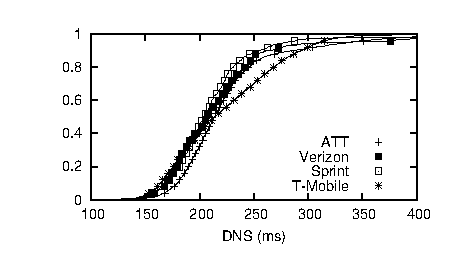
\includegraphics[width=0.4\textwidth]{figures/web_real/dns.eps}
%\caption{CDF of DNS lookup time on all platforms} \label{fig:dns}
%\end{figure}

	
\nsection{Other Mobile Applications}
\label{sec:other}


In this section, we study two other popular mobile applications, streaming video and VoIP.

Streaming video is another popular application on smartphones. We measure streaming video performance by playing a 37:40~minute video on the phones using the YouTube application. From the collected packet trace, we calculate the downloading size of the video by adding up the payloads for all the packets from the server to phone while excluding the retransmitted packets. 

\begin{figure*}[t]
\centering
\begin{tabular}{cc}
\multicolumn{2}{c}{\IGM{figures/mobisys10/videosize.eps}}\\
\multicolumn{2}{c}{(a) Video content size} \\
\IGM{figures/mobisys10/iphonetimeline.eps}&
\IGM{figures/mobisys10/gphonetimeline.eps}\\
(b) iPhone timeline for 2260-sec video &
(c) G2 timeline for 2260-sec video \\
\end{tabular}
\ncaption{Streaming video performance: content size, download strategy}
\label{fig:video}
\end{figure*}


%Streaming media are multimedia that are constantly received by, and normally presented to,
%an end-user while being delivered by a streaming provider. Streaming media can be Live media or
%On demand media. We only concentrate on On demand streaming video in this paper. Playing a streaming
%video on the client has two phases, downloading the video and processing the video to display it to the
%user. Both these phases run in parallel. Since the size of streaming video is very large so network throughput 
%is an important factor in determining the streaming video performance. Different streaming players use network 
%layer protocols download the video\eg TCP, UDP, RTSP \etc We only look at TCP in this paper.
%Client execution speed is another important factor which affects the performance of streaming media. 
%It is important to study the effect of all these factors to determine the bottleneck in performance.
%Unfortunately, due to lack of time we only made some preliminary observations regarding streaming video
%application performance.

\nsubsection{Streaming video}\label{sec:video}

We downloaded a 37-minute long video using a YouTube player on 
each phone. Figure~\ref{fig:video}(a) shows the size of the video
downloaded using TCP via WiFi and 3G on each phone. As expected, 
the video size is smaller for 3G than for WiFi, because both the 
video server and 3G carrier can customize video based on network 
conditions to ensure good user experience. Interestingly, the video 
size for 3G also varies across carriers: it is the smallest for 
T-Mobile, followed by AT\&T, Verizon, and Sprint. 
%Since different carriers
%download different content for the same video, streaming video
%performance can be highly variable across different carriers.

Figures~\ref{fig:video}(b)(c) show the representative time series 
of video download throughput for iPhone and G2 via 3G networks.
The timeline of iPhone exhibits a distinct pattern with clear pauses. 
It initially downloads a portion of the video at a high rate, then 
stops before downloading the remaining portions. We conjecture that 
the download stops when the buffered content exceeds a certain 
threshold, and resumes after the buffered content falls below another 
threshold. The purpose is likely to accommodate the limited phone
memory and to save energy usage associated with the 3G interface. 
Another observation is that iPhone always terminates the TCP 
connection every 10--20 seconds and then establishes a new one on 
demand. We conjecture that iPhone attempts to put the 3G 
interface into low power state to save energy. 

In contrast, G2 shows a different behavior by periodically 
downloading small chunks of the video every 10 seconds. The Samsung 
and Palm phones behave similarly with a slightly longer interval of 
20 seconds between downloads. This is likely motivated by the fact 
that users sometimes do not watch the entire video and may skim 
through certain parts of the video. Such downloading patterns can 
also help conserve energy. Our initial study shows that the video 
players on different phones employ different policies to fetch video. 
This merits more detailed future study. 

%constraints in energy and memory. 

%while trying to satisfy resource
%\begin{figure}[t]
%\centering
%\caption{Video content size comparison}
%\label{fig:video_size}
%\end{figure}




\nsubsection{VoIP}\label{sec:voip}

%\begin{figure*}[t]
%\begin{tabular}{cc}
%\centering
%\includegraphics[width=0.45\textwidth]{figures/voip/voip_inter.eps} &
%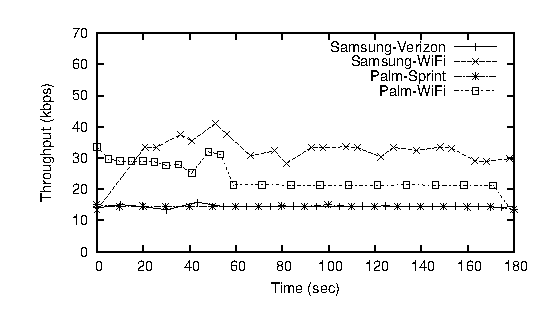
\includegraphics[width=0.45\textwidth]{figures/voip/voip_thru.eps} \\
%\small{(a) CDFs of the inter-packet arrival time and inter-packet departure time} &
%\small{(b) Downlink throughput varies with time} \\
%\end{tabular}
%\caption{VoIP performance} \label{fig:voip}
%\end{figure*}

%We use a popular VoIP application to call a wired computer from a 
%smartphone and play a piece of clip on both sides simulating 


We carry out a simple VoIP experiment on the Samsung (Verizon) and 
Palm (Sprint) phones given their uniform support for Skype. During 
the experiment, the same 3-minute music file is played on both the phone and 
the desktop, when the two are in a Skype call. The volume is kept 
the same to have similar voice input. Figure~\ref{fig:voip} shows 
that the throughput for both phones via 3G is nearly identical, as 
the same coding rate is used. The throughput is higher under WiFi 
than under 3G, as different amount of data is transferred depending 
on the network being used. This reflects how Skype tries to vary 
the encoding rate according to the network condition to achieve 
good perceived voice quality.


%Figure~\ref{fig:voip}(a) shows the inter-arrival time and inter-departure time from which we can study the difference originated from the platform. The inter-arrival time is the interval between two packets from our desktops to our phones, while the inter-departure time is the interval between two packets from our phones to our desktops. The only difference between inter-arrival time and inter-departure time is the platform that originates the traffic. However, from Figure~\ref{fig:voip}(a), we cannot say which one between the inter-arrival and inter-departure is better. The inter-packet arrival time of the Samsung phone is longer than its inter-departure, which is on the contrary on the Sprint phone. Figure~\ref{fig:voip_}(a) at least indicates that phone's processing ability is not the bottleneck for VoIP service.

%In all, in our experiments, platform is not the bottleneck, but the network condition may affect the performance in terms of payload size. When the phone is using WiFi, the throughput is consistently higher than that in 3G. 
%



\begin{figure}[t]
\centering
%\includegraphics[width=0.45\textwidth]{figures/voip/voip_inter.eps} &
\IG{figures/mobisys10/voip_thru.eps} \\
%\small{(a) CDFs of the inter-packet arrival time and inter-packet departure time} &
\small{Downlink throughput timeline for Skype} \\
\ncaption{VoIP performance} \label{fig:voip}
\end{figure}


